% latex2e header
\documentclass[11pt]{article}
\usepackage{latexsym}
\usepackage{fullpage}
\usepackage{graphicx}

\setlength{\textheight}{10.0in}
\begin{document}
\thispagestyle{empty}

{\bf Spring 2015 EECS192 Mechatronics Design Laboratory Oral Presentations }\\

Thu. Apr. 30, 9-1130 am (289 Cory) / Fri. May 1, 1130-200 pm (540AB Cory)

The purpose of the oral presentation is to provide you with an
opportunity to inform your peers about what made your car successful.
Due to the size of the class, each group's presentation will
need to be no more than 9 minutes with two minutes left for
answering questions and changeover. 
Be sure to practice and time your presentation.
Assume that your audience is very familiar with the project.  Hence, you do
not need to explain how the line camera sensors work or how the program
is compiled.

Power Point can be used to clearly convey your ideas to the class.
Typically, going through ten slides in ten minutes is about right.
Hand in (2) paper copies of your slides (2 up) at beginning of class on
Thu. Apr. 30. The following items should be addressed during your
presentation:\\

1.  Vehicle Electronic and Mechanical Hardware (15 \%)\\
Show a basic block diagram with major hardware subsystems.
What is different about your hardware (basic electronics/wiring)? 
Briefly note mechanical
issues such as mounting boards, camera, vibration, suspension issues, etc.
Include photos to illustrate features.
What are the
advantages and disadvantages your methods? 
Some items that you might want to consider are cost, complexity,
reliability, and accuracy.\\ 

2.  Software (20\%)\\
Provide an overview block diagram of your software.
Describe organization (with a picture) of threads, tasks, timing etc.
Note update rates for various processes.
What is unique about your software?  For example, do
you use auto calibration of sensors, course memorization, automatic
determination of gain constants for the controls, etc.?
How did you make your line sensing robust?\\

3.  Controls (15\%)\\
What kind of stability problems did you have and how
did you overcome them?  State how you
implemented the controller and how you chose the gain constants.
What gains were used (radians per meter, radians/(m/sec) )? 
Did simulation provide any help?\\

4.  How well did it work? (20\%)\\
\begin{tabular}{lr}
\parbox[b]{3.5in}{Record the lateral error, including waterfall plots,
during a run at speed starting on the straight section on the
track as shown to the right. Plot lateral error
versus time (and velocity versus time, if available). 
Be sure to note your velocity (m/s).
Explain from the plots where 
the control system would allow the car to
go faster, or where the car is at some stability limit.}
~~ & 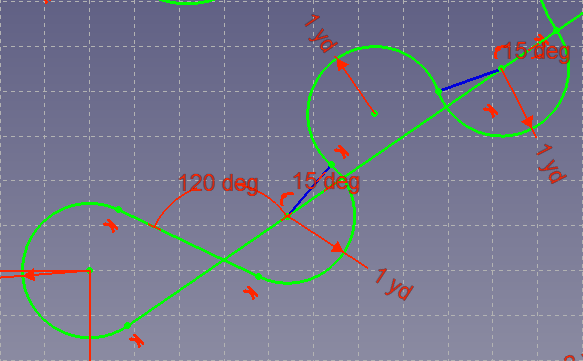
\includegraphics[scale=0.4]{track_slalom.png}\\
\end{tabular}
\vspace{0.1in}

5. Lessons learned (25\%)\\
What were your most memorable glitches, failures or debugging issues?\\
What tools did you use- e.g. telemetry, autotuning, custom tools, simulation?
What didn't you know that you needed to know?\\
Advice for next year's class?\\

6. Roles and Contributions (5\%)\\
Briefly describe the role of each team member.\\

%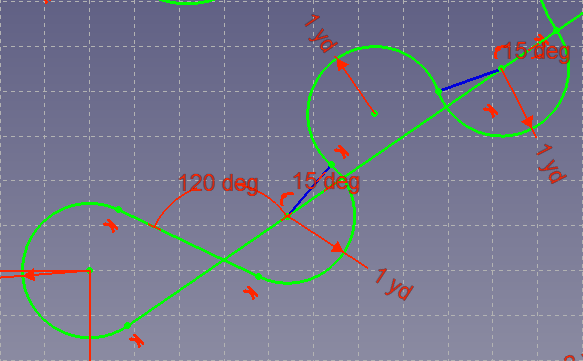
\includegraphics[scale=0.4]{track_slalom.png}

\end{document}
